\documentclass[13pt,a4paper]{article}
\usepackage[spanish,es-nodecimaldot]{babel}	% Utilizar español
\usepackage[utf8]{inputenc}					% Caracteres UTF-8
\usepackage{graphicx}						% Imagenes
\usepackage[hidelinks]{hyperref}			% Poner enlaces sin marcarlos en rojo
\usepackage{fancyhdr}						% Modificar encabezados y pies de pagina
\usepackage{float}							% Insertar figuras
\usepackage[textwidth=390pt]{geometry}		% Anchura de la pagina
\usepackage[nottoc]{tocbibind}				% Referencias (no incluir num pagina indice en Indice)
\usepackage{enumitem}						% Permitir enumerate con distintos simbolos
% \usepackage[T1]{fontenc}					% Usar textsc en sections
\usepackage{amsmath}						% Símbolos matemáticos
\usepackage[ruled,vlined]{algorithm2e}      % Pseudocódigo
\usepackage{xcolor}
\usepackage{listings}
% Para que acepten tíldes los listing
\lstset{     
     literate=%
         {á}{{\'a}}1
         {é}{{\'e}}1
         {í}{{\'i}}1
         {ó}{{\'o}}1
         {ú}{{\'u}}1
         {Á}{{\'A}}1
         {É}{{\'E}}1
         {Í}{{\'I}}1
         {Ó}{{\'O}}1 
         {Ú}{{\'U}}1
         {ñ}{{\~n}}1 
         {Ñ}{{\~N}}1 
         {¿}{{?``}}1 
         {¡}{{!``}}1
}
\usepackage{dsfont}
\usepackage{caption, subcaption}

% ==============================================================================

\usepackage{caption}
\usepackage[section]{placeins}
\makeatletter
\def\fps@figure{H}
\makeatother

\usepackage{booktabs}
\usepackage{longtable}
\usepackage{array}
\usepackage{multirow}
\usepackage{wrapfig}
\usepackage{colortbl}
\usepackage{pdflscape}
\usepackage{tabu}
\usepackage{threeparttable}
\usepackage{threeparttablex}
\usepackage[normalem]{ulem}
\usepackage{makecell}
\usepackage[bottom]{footmisc}

% ==============================================================================
% ==============================================================================

% Comando para poner el nombre de la asignatura
\newcommand{\asignatura}{TSCAO}
\newcommand{\autor}{Ignacio Vellido Expósito}
\newcommand{\email}{ignaciove@correo.ugr.es}
\newcommand{\titulo}{Optimización}
\newcommand{\subtitulo}{Trabajo final}

% Configuracion de encabezados y pies de pagina
\pagestyle{fancy}
\lhead{\autor{}}
\rhead{\asignatura{}}
\lfoot{Máster Ciencia de Datos e Ingeniería de Computadores}
\cfoot{}
\rfoot{\thepage}
\renewcommand{\headrulewidth}{0.4pt}		% Linea cabeza de pagina
\renewcommand{\footrulewidth}{0.4pt}		% Linea pie de pagina

% ==============================================================================
% ==============================================================================

\begin{document}
    \pagenumbering{gobble}
    % ==============================================================================
% Pagina de titulo
\begin{titlepage}
    \begin{minipage}{\textwidth}
        \centering

        
\includegraphics[scale=0.5]{img/ugr.png}\\

        \textsc{\Large \asignatura{}\\[0.2cm]}
        \textsc{MÁSTER CIENCIA DE DATOS E INGENIERÍA DE COMPUTADORES}\\[1cm]

        \noindent\rule[-1ex]{\textwidth}{1pt}\\[1.5ex]
        \textsc{{\Huge \titulo\\[0.5ex]}}
        \textsc{{\Large \subtitulo\\}}
        \noindent\rule[-1ex]{\textwidth}{2pt}\\[2.5ex]

        \end{minipage}

        \vspace{0.3cm}

        \begin{minipage}{\textwidth}

        \centering

        \textbf{Autor}\\ {\autor{} \\ ignaciove@correo.ugr.es}\\[1.5ex]
        \vspace{0.4cm}

        
\includegraphics[scale=0.3]{img/etsiit.jpeg}
        
\includegraphics[scale=0.6]{img/master.png}

        \vspace{0.7cm}
        \textsc{Escuela Técnica Superior de Ingenierías Informática y de Telecomunicación}\\
        \vspace{1cm}
        \textsc{Curso 2020-2021}
    \end{minipage}
\end{titlepage}
% ==============================================================================
    
    \pagenumbering{arabic}    
    \newpage

    % ==============================================================================

\section{Parte 1}

\textbf{El problema de los árboles frutales}

\vspace{\baselineskip}

Un agricultor dispone de una superficie de 640m² para cultivar naranjos, perales, manzanos y
limoneros. La cuestión es cómo debe distribuir la superficie entre los árboles para maximizar
los beneficios teniendo la siguiente información:

\begin{itemize}
    \item Los naranjos necesitan un mínimo de 16m², los perales necesitan 4m², los manzanos 8m² y cada limonero necesita 12m².
    \item El agricultor dispone de 900 horas de trabajo al año. Las demandas de los diferentes árboles son: cada naranjo 30 horas, cada peral 5 horas, cada manzano 10 horas y cada limonero 20 horas.
    \item Debido a las restricciones, el agua disponible para el riego es de 200m³ al año. La demanda de agua (por año y árbol) es: naranjo: 2m³, peral 3m³, manzano: 1m³ y limonero 2m³.
    \item Los beneficios (por año y árbol) son de 50, 25, 20 y 30 euros para los naranjos, perales, manzanos y limoneros respectivamente.
\end{itemize}

\vspace{\baselineskip}

Se plantea el problema de la siguiente forma:
\begin{lstlisting}[mathescape=true]
    N = Número de naranjos
    M = Número de manzanos
    L = Número de limoneros
    P = Número de perales

    max    50N + 25P + 20M + 30L 
    s.t.   16N +  4P +  8M + 12L $\leq$ 640
           30N +  5P + 10M + 20L $\leq$ 900
            2N +  3P +   M +  2L $\leq$ 200
             N,    P,    M,    L $\geq$   0
\end{lstlisting}

\begin{figure}[t]\center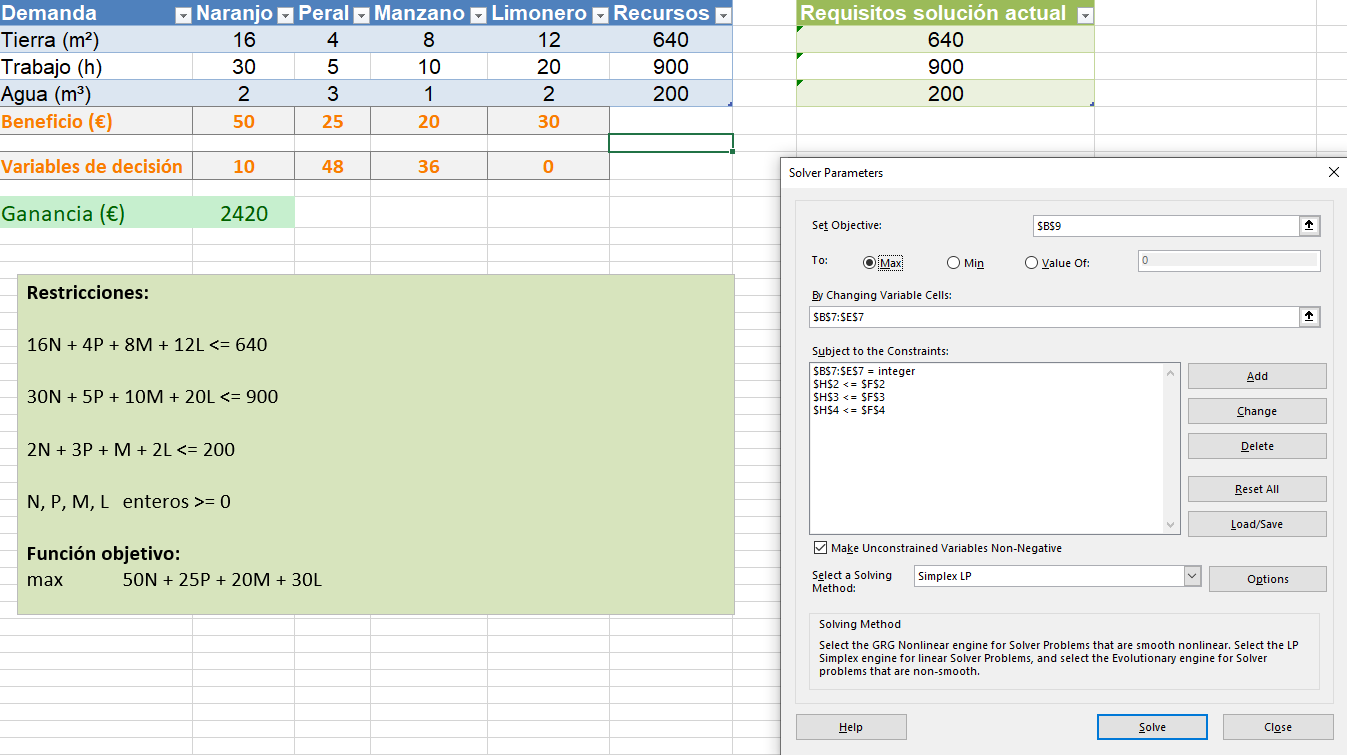
\includegraphics[width=.95\linewidth]{img/solver.png}\caption{Resolución del problema de los árboles frutales.}\end{figure}

\begin{figure}[b]\center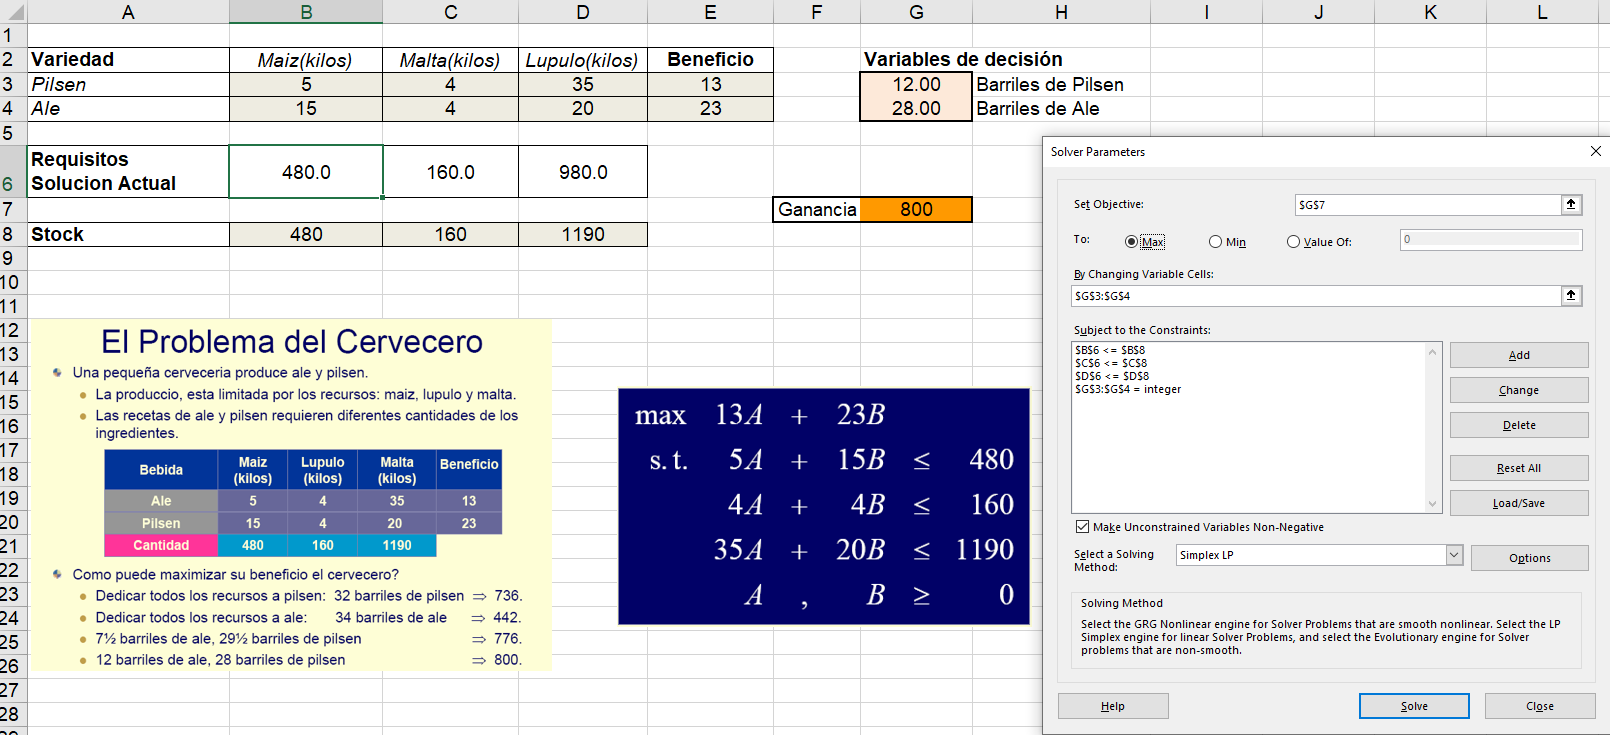
\includegraphics[width=.95\linewidth]{img/solver2.png}\caption{Resolución del problema de la cervecería.}\end{figure}

\begin{figure}[t]\center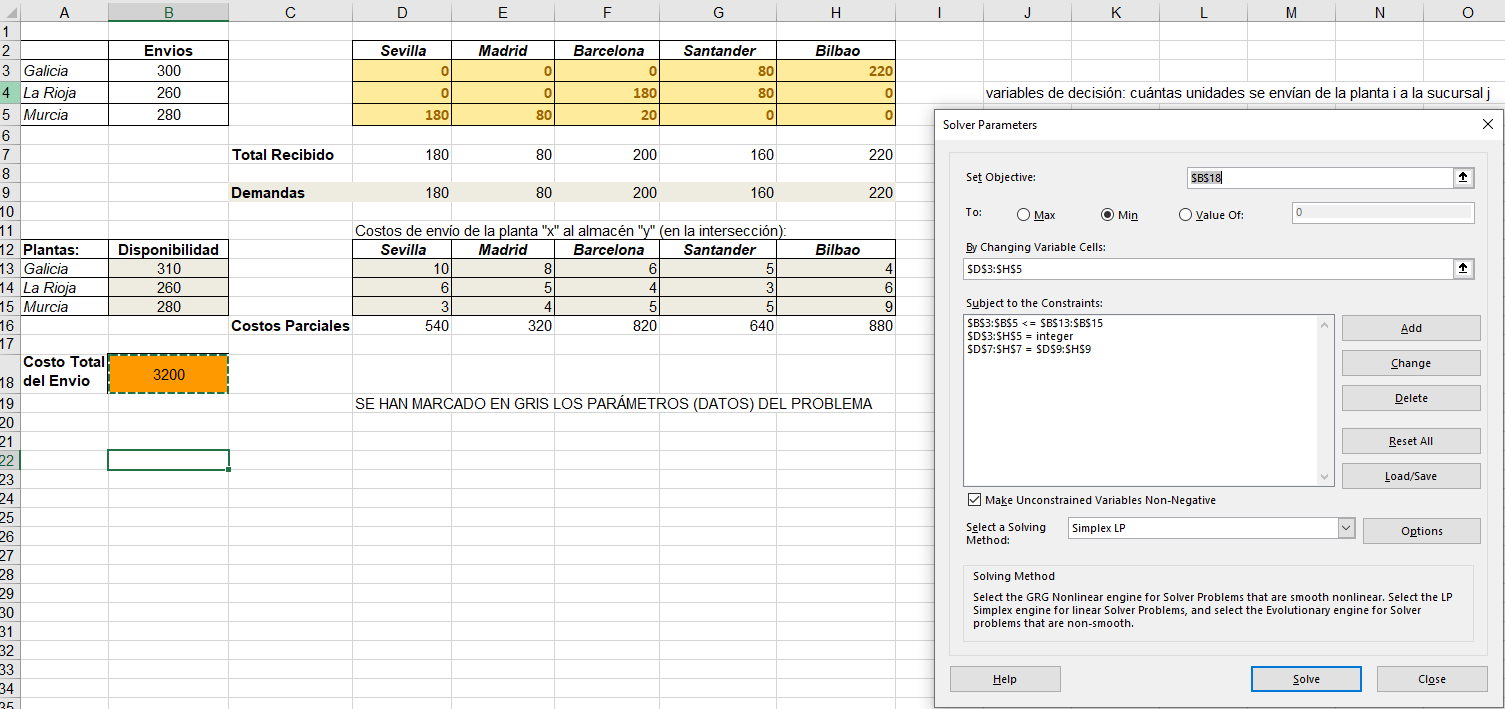
\includegraphics[width=.95\linewidth]{img/solver3.png}\caption{Resolución del problema de la distribución de mercancías.}\end{figure}

\newpage

\section{Parte 2}

\begin{figure}[H]
    \centering
    \resizebox{0.75\columnwidth}{!}{%
    \begin{tabular}{| l || c | c | c |} 
        \hline
        \textbf{Heurística} & \multicolumn{3}{c |}{\textbf{Problema}} \\
        \Xhline{2\arrayrulewidth}
        & bcl380 & icw1483 & bck2217 \\
        \hline
        Greedy & 1862 & 5032 & 7851 \\
        \hline
        Borukva & 1915 & 5166 & 7861 \\
        \hline
        Quick Borukva & 1872 & 5379 & 8117 \\
        \hline
        Nearest Neighbour & 2057 & 5681 & 8740 \\
        \hline
        Lin Kernighan Default (+ Greedy) & 1644 & 4487 & 6848 \\
        \hline
        Lin Kernighan 10 kicks & 1668 & 4738 & 7196 \\
        \hline
        Lin Kernighan 100 kicks & 1634 & 4601 & 7098 \\
        \hline
        Lin Kernighan + Quick Borukva & 1630 & 4501 & 6910 \\
        \hline
        Random & 26086 & 149247 & 297518 \\
        \hline
    \end{tabular}
    }
    \caption{Resultados de distancia de cada heurística para los diferentes problemas TSP.}
\end{figure}

Lin Kernighan obtiene los mejores resultados para cada uno de los problemas, a costa de un mayor tiempo de cómputo. Entre el resto (y a excepción de Nearest Neighbour) no existen diferencias suficientemente significas en la calidad de las soluciones encontradas, aunque la heurística Greedy es la que obtiene mejores resultados en estas instancias de TSP.

\vspace{\baselineskip}

Los cambios en los parámetros de la heurística Lin Kernighan dan resultados inconsistentes, pero apreciamos que el decremento del número de ``kicks'' (por defecto igual al número de nodos) influye negativamente en la longitud de los caminos encontrados.

También notamos que el cambio del algoritmo inicial afecta en tiempo de cómputo pero apenas en los resultados obtenidos, siendo en general ligeramente inferiores pasando de Greedy a Quick Borukva.

\begin{figure}[b]
    \centering 
    \begin{subfigure}[t]{0.3\textwidth}
      \centering
      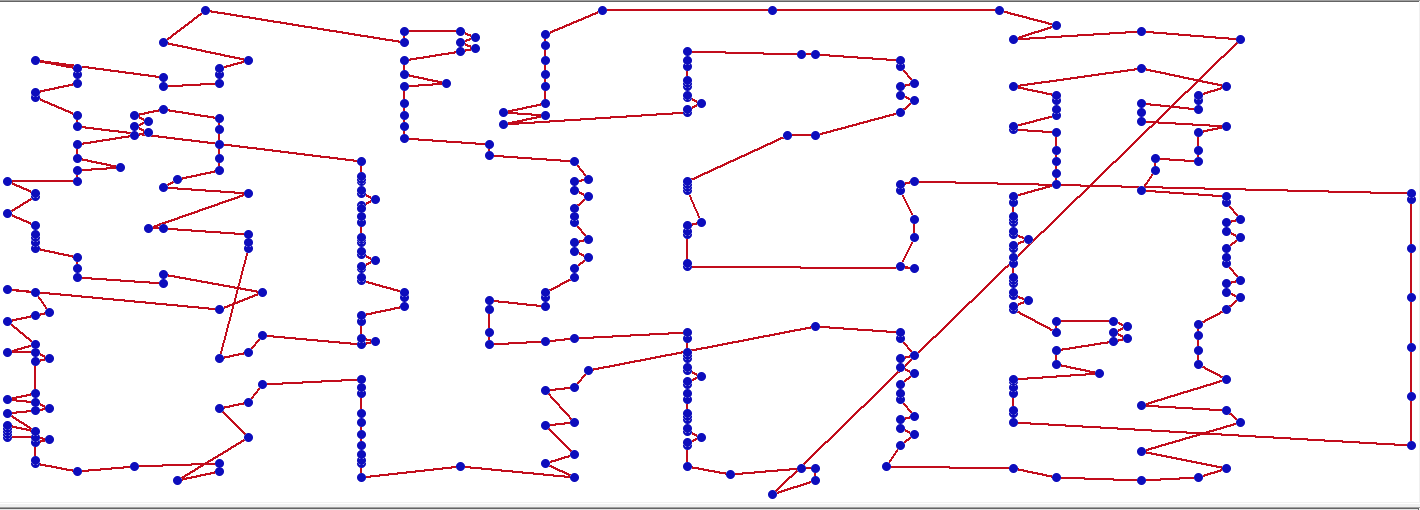
\includegraphics[width=\textwidth]{img/1/G.png}
      \caption{Greedy.}
    \end{subfigure}
    % \vspace{7mm}
    % \hfill
    \begin{subfigure}[t]{0.3\textwidth}
        \centering
        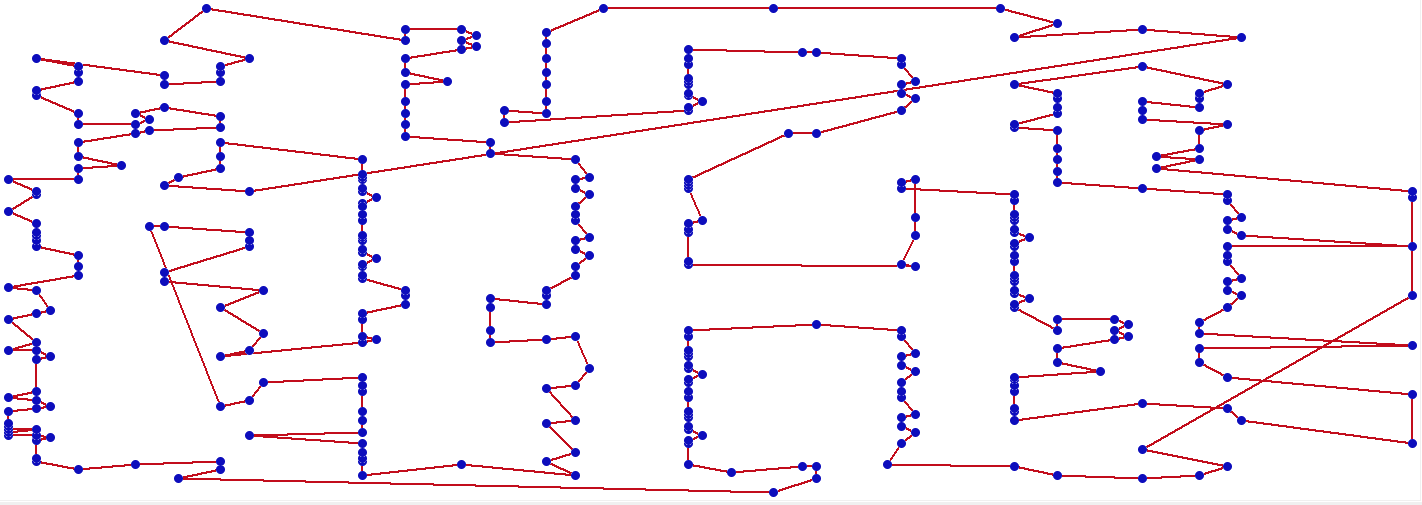
\includegraphics[width=\textwidth]{img/1/B.png}
        \caption{Borukva.}
    \end{subfigure}
    % \hfill
    \begin{subfigure}[t]{0.3\textwidth}
      \centering
      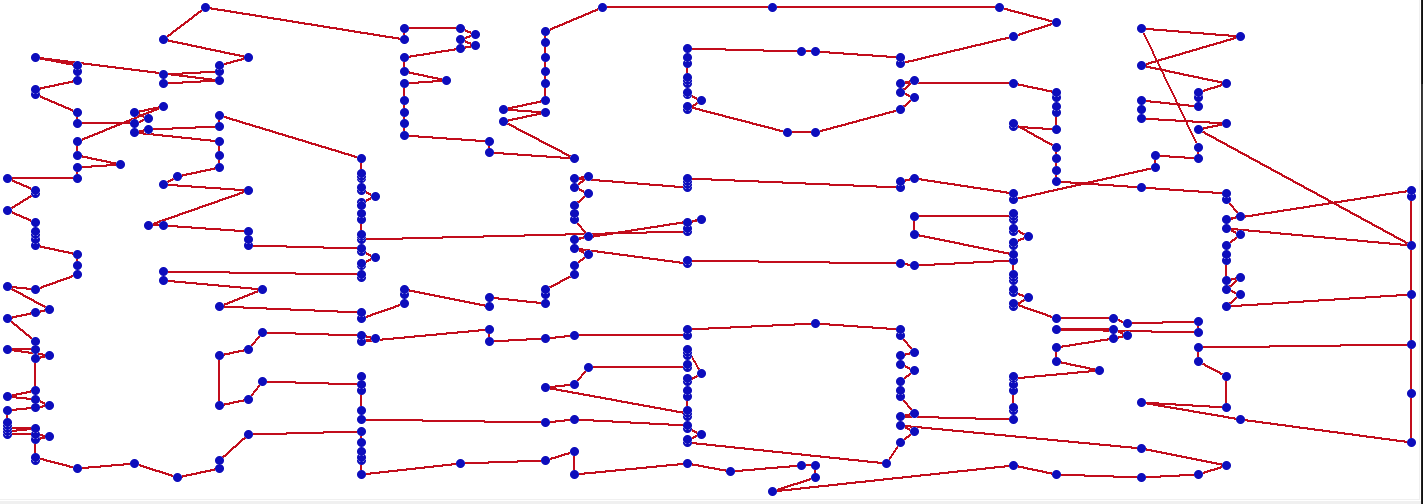
\includegraphics[width=\textwidth]{img/1/Q.png}
      \caption{Quick Borukva.}
    \end{subfigure}

    % \hfill
    \begin{subfigure}[t]{0.3\textwidth}
        \centering
        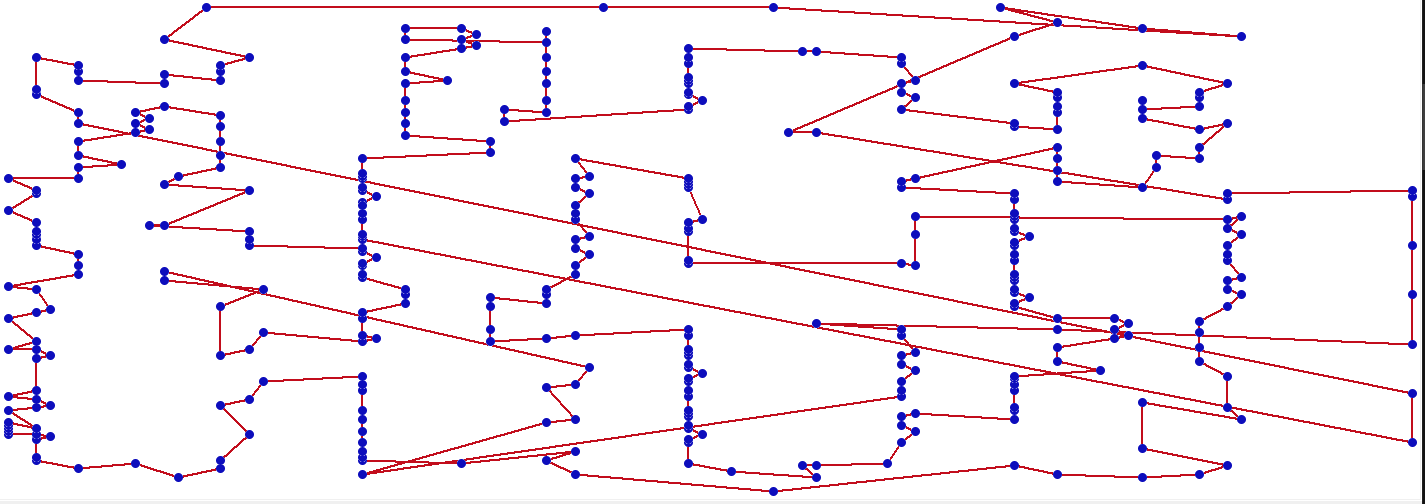
\includegraphics[width=\textwidth]{img/1/N.png}
        \caption{Nearest Neighbour.}
    \end{subfigure}
    % \hfill
    \begin{subfigure}[t]{0.3\textwidth}
        \centering
        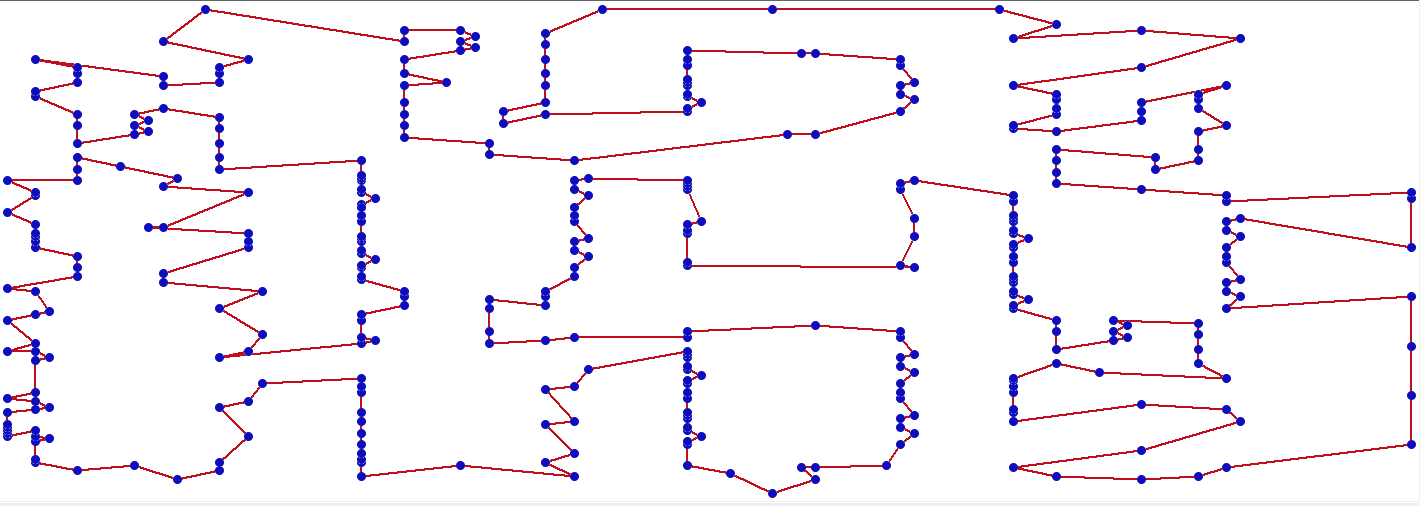
\includegraphics[width=\textwidth]{img/1/L1.png}
        \caption{Lin Kernighan Default.}
    \end{subfigure}
    % \hfill
    \begin{subfigure}[t]{0.3\textwidth}
        \centering
        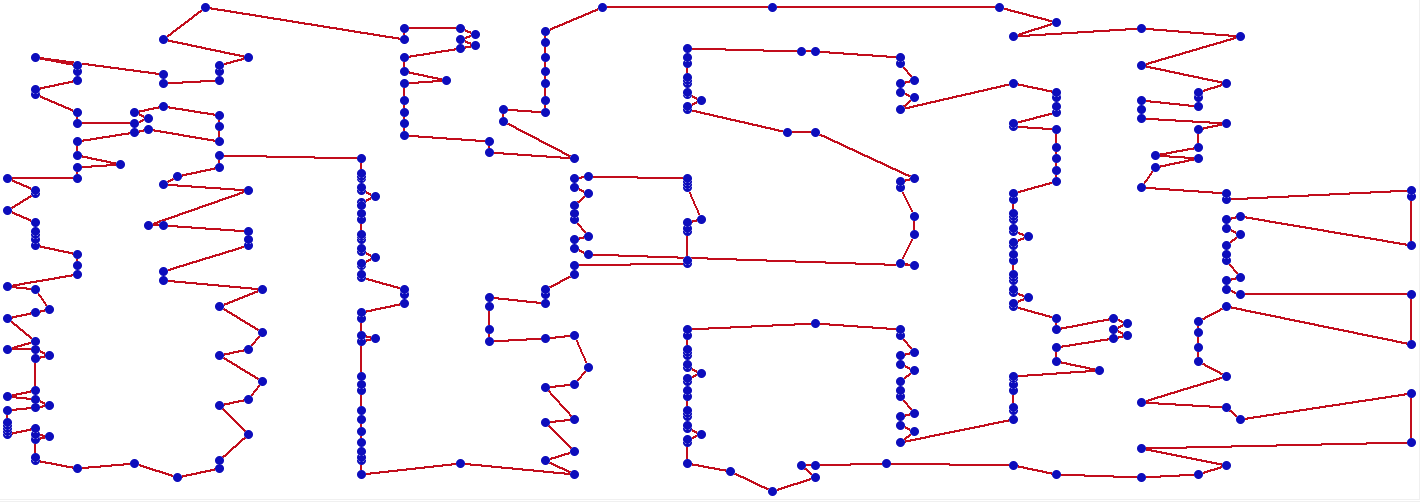
\includegraphics[width=\textwidth]{img/1/L10.png}
        \caption{Lin Kernighan 10 kicks.}
    \end{subfigure}

    % \hfill
    \begin{subfigure}[t]{0.3\textwidth}
        \centering
        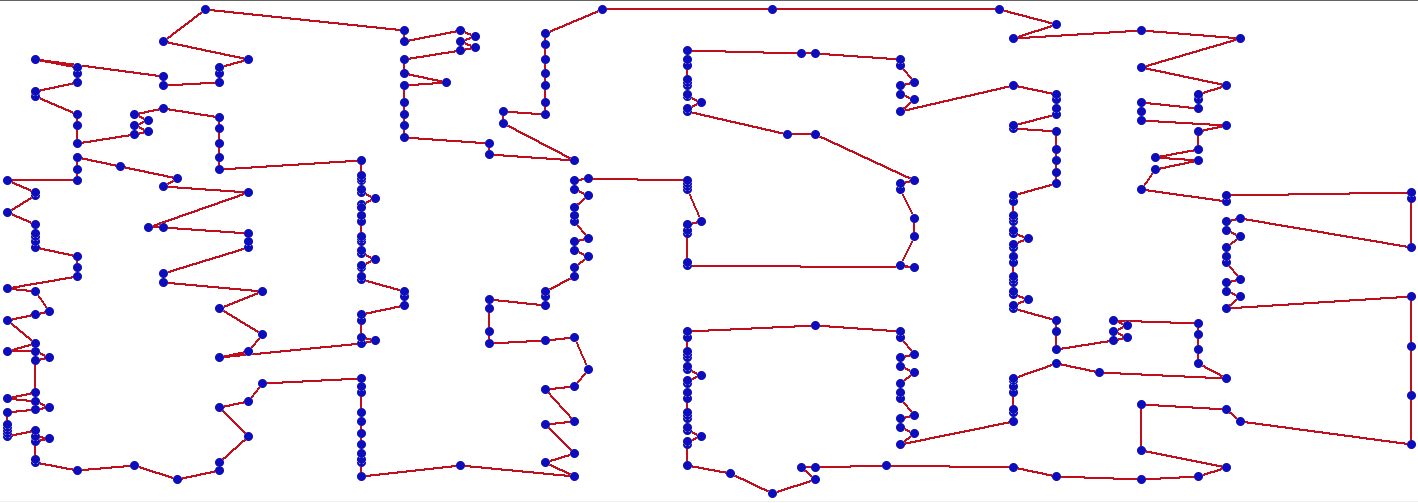
\includegraphics[width=\textwidth]{img/1/L100.png}
        \caption{Lin Kernighan 100 kicks.}
    \end{subfigure}
    % \hfill
    \begin{subfigure}[t]{0.3\textwidth}
        \centering
        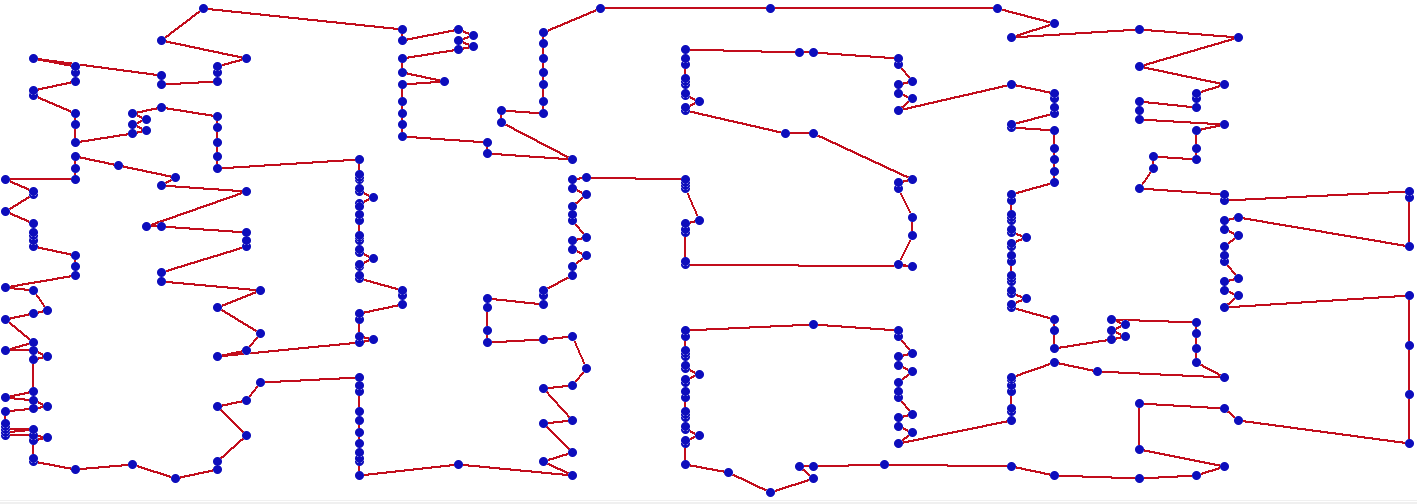
\includegraphics[width=\textwidth]{img/1/L+Q.png}
        \caption{L.K + Quick Borukva.}
    \end{subfigure}
    % \hfill
    \begin{subfigure}[t]{0.3\textwidth}
        \centering
        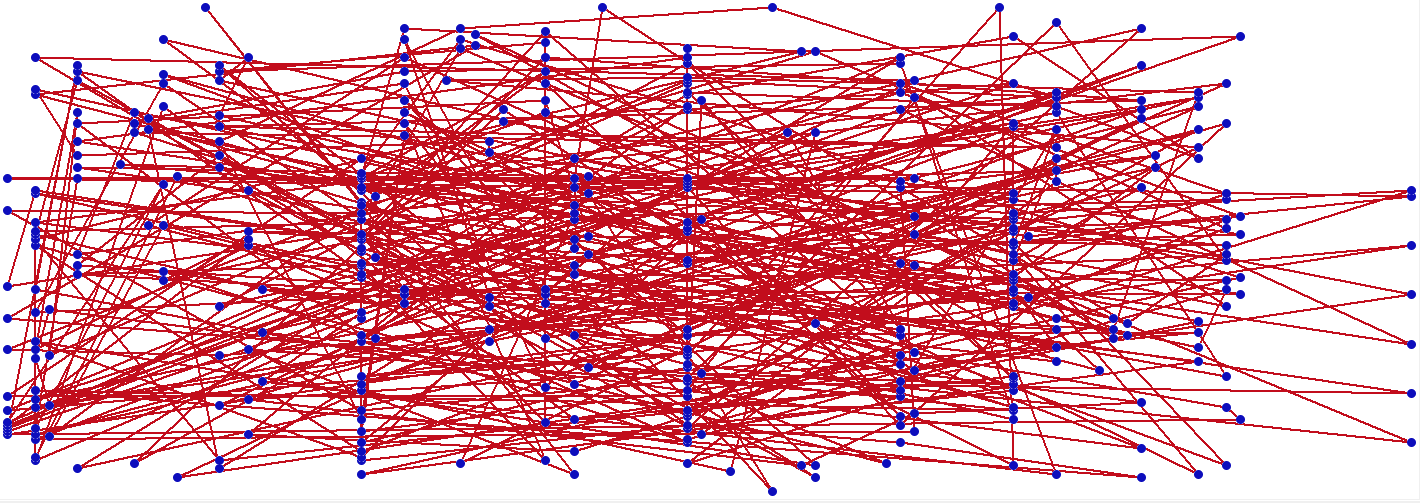
\includegraphics[width=\textwidth]{img/1/R.png}
        \caption{Random.}
    \end{subfigure}
    \caption{Rutas calculadas por cada heurística para el problema bcl380.}
\end{figure}
  
\begin{figure}[t]
    \centering 
    \begin{subfigure}[t]{0.3\textwidth}
      \centering
      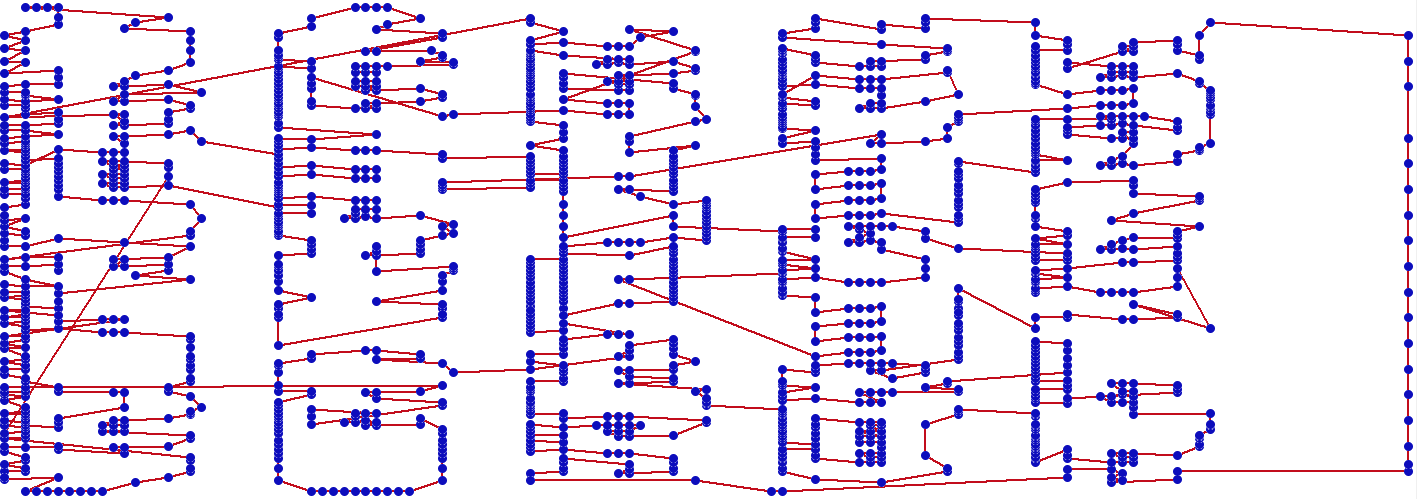
\includegraphics[width=\textwidth]{img/2/G.png}
      \caption{Greedy.}
    \end{subfigure}
    % \vspace{7mm}
    % \hfill
    \begin{subfigure}[t]{0.3\textwidth}
        \centering
        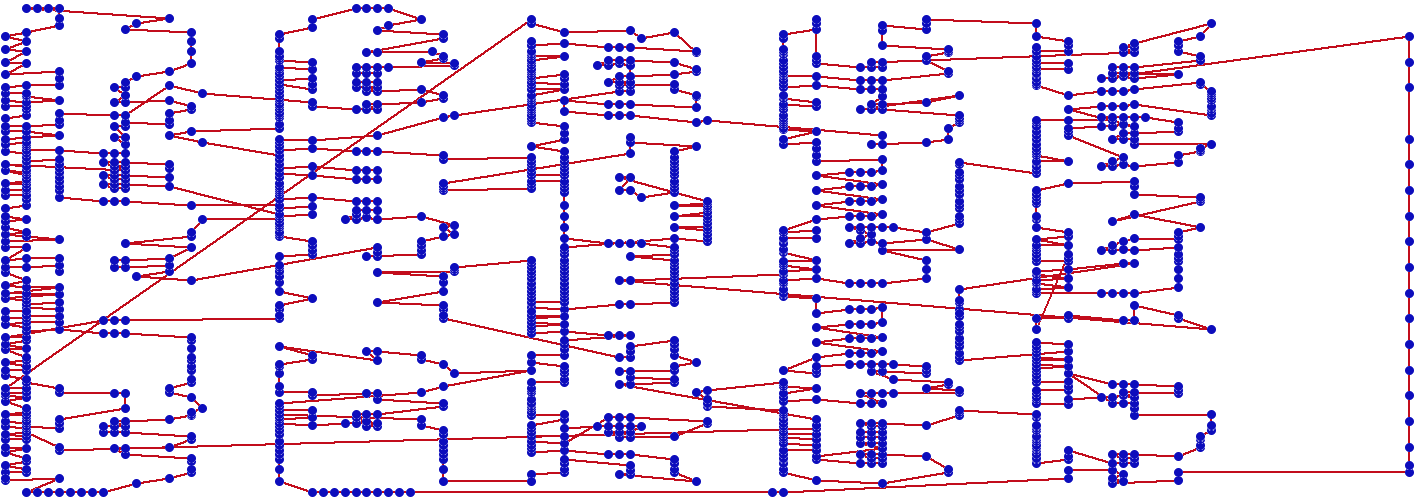
\includegraphics[width=\textwidth]{img/2/B.png}
        \caption{Borukva.}
    \end{subfigure}
    % \hfill
    \begin{subfigure}[t]{0.3\textwidth}
      \centering
      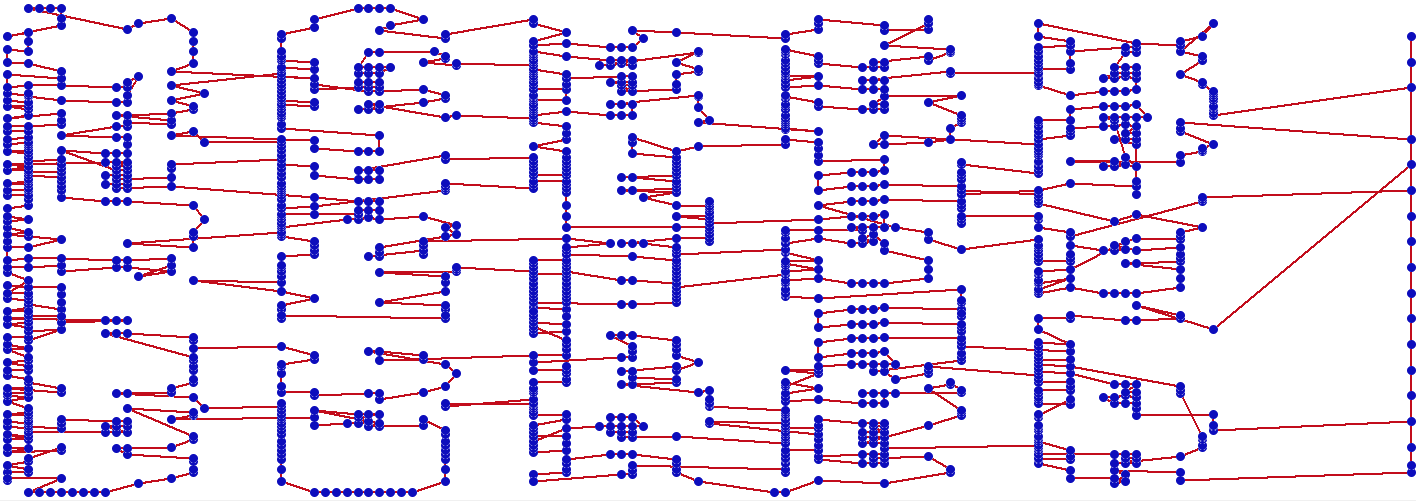
\includegraphics[width=\textwidth]{img/2/Q.png}
      \caption{Quick Borukva.}
    \end{subfigure}

    % \hfill
    \begin{subfigure}[t]{0.3\textwidth}
        \centering
        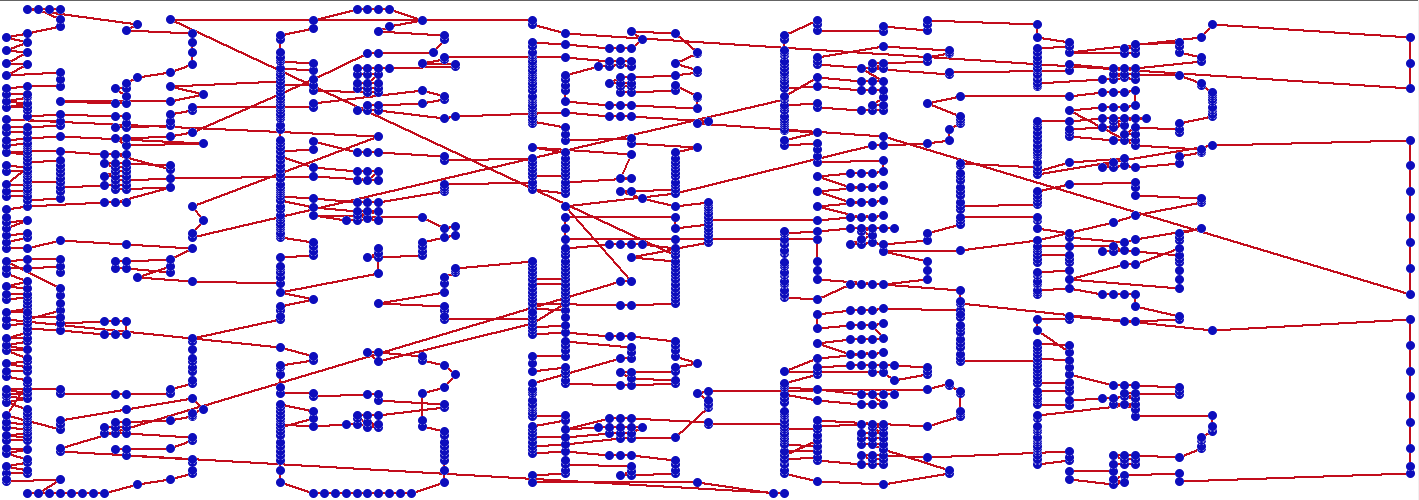
\includegraphics[width=\textwidth]{img/2/N.png}
        \caption{Nearest Neighbour.}
    \end{subfigure}
    % \hfill
    \begin{subfigure}[t]{0.3\textwidth}
        \centering
        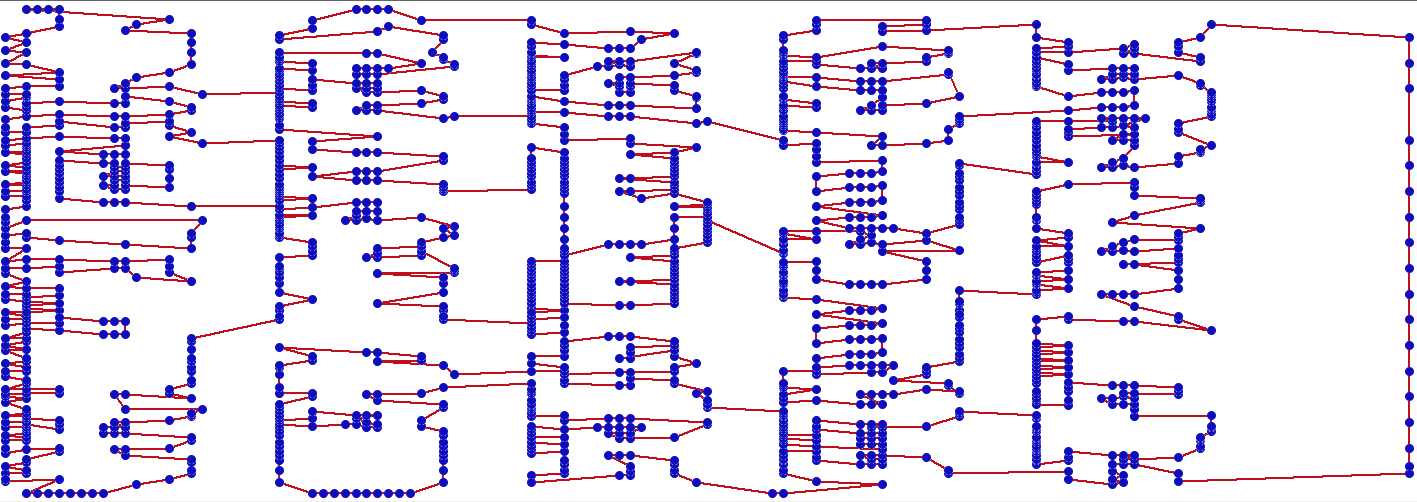
\includegraphics[width=\textwidth]{img/2/L1.png}
        \caption{Lin Kernighan Default.}
    \end{subfigure}
    % \hfill
    \begin{subfigure}[t]{0.3\textwidth}
        \centering
        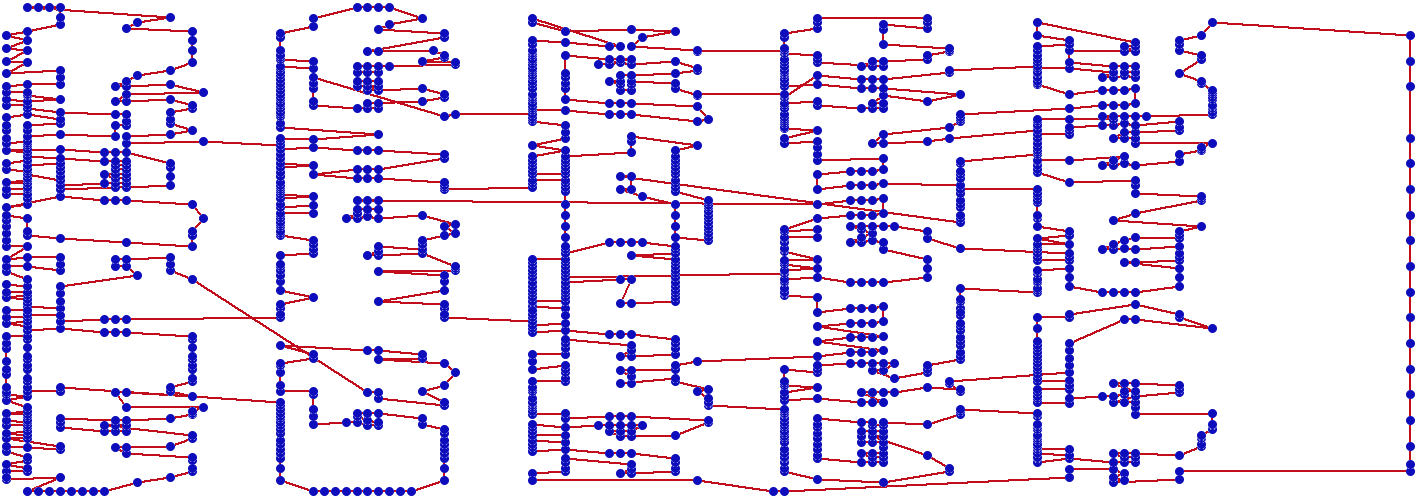
\includegraphics[width=\textwidth]{img/2/L10.png}
        \caption{Lin Kernighan 10 kicks.}
    \end{subfigure}

    % \hfill
    \begin{subfigure}[t]{0.3\textwidth}
        \centering
        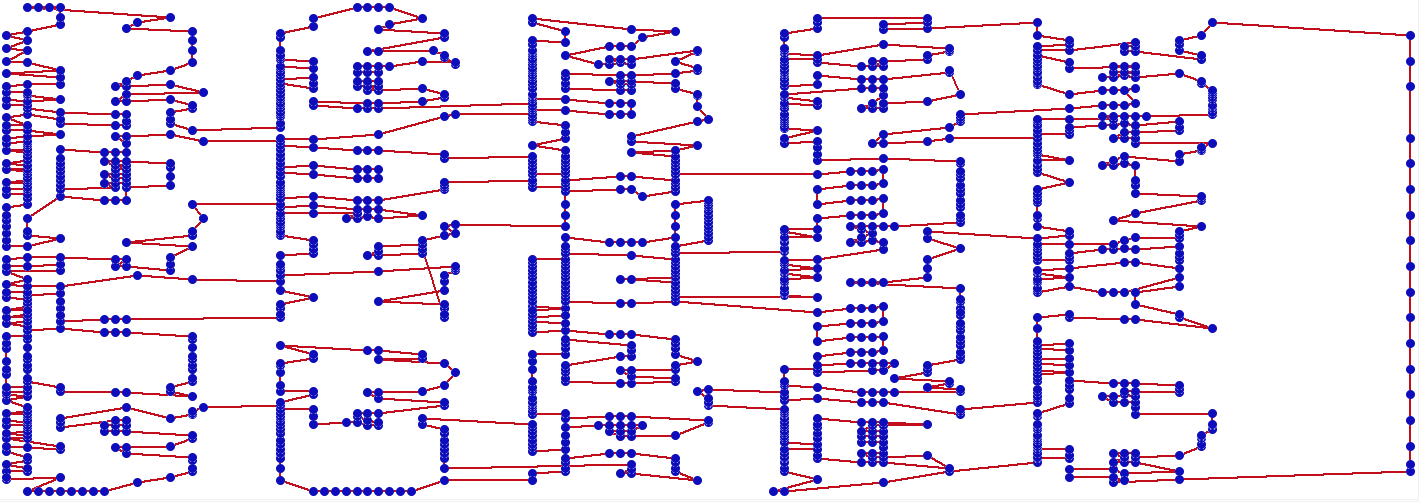
\includegraphics[width=\textwidth]{img/2/L100.png}
        \caption{Lin Kernighan 100 kicks.}
    \end{subfigure}
    % \hfill
    \begin{subfigure}[t]{0.3\textwidth}
        \centering
        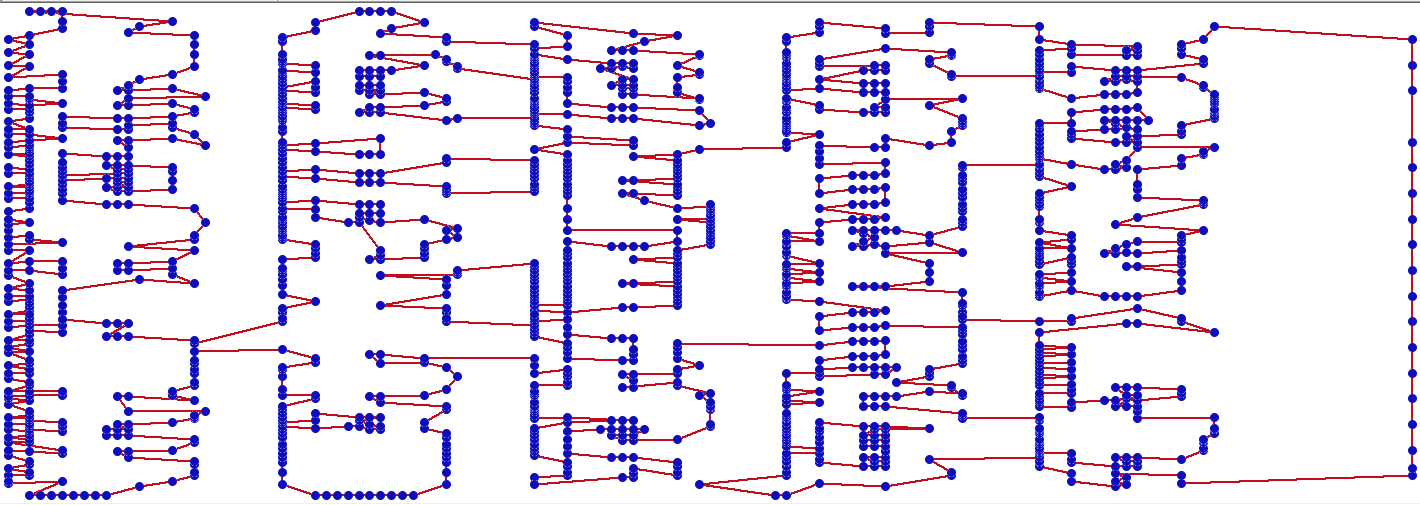
\includegraphics[width=\textwidth]{img/2/L+Q.png}
        \caption{L.K + Quick Borukva.}
    \end{subfigure}
    % \hfill
    \begin{subfigure}[t]{0.3\textwidth}
        \centering
        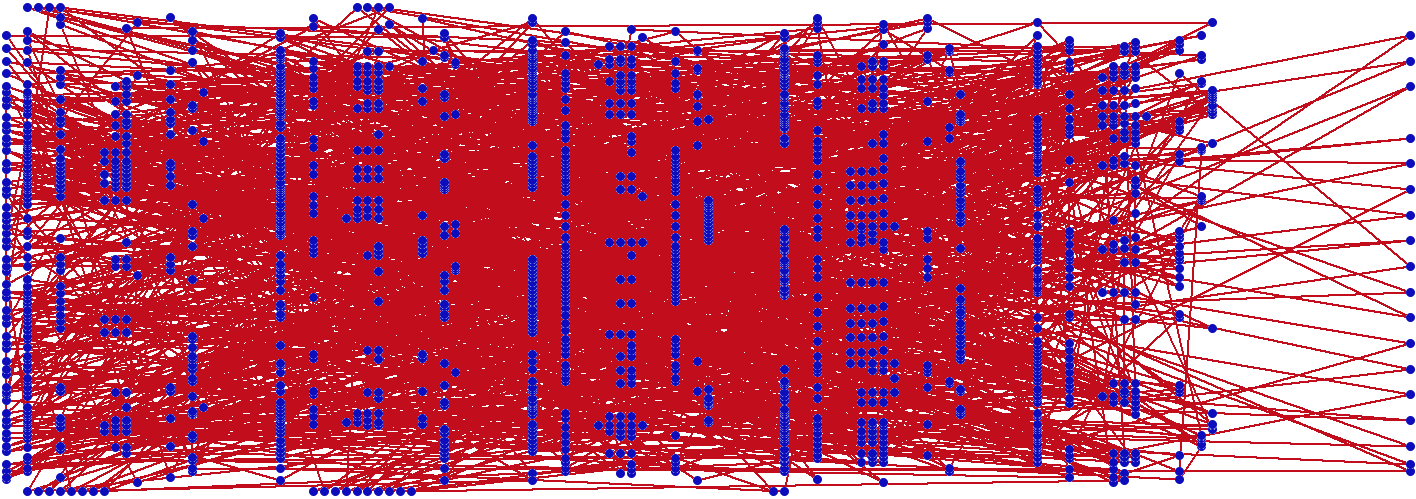
\includegraphics[width=\textwidth]{img/2/R.png}
        \caption{Random.}
    \end{subfigure}
    \caption{Rutas calculadas por cada heurística para el problema icw1483.}
\end{figure}


\begin{figure}[b]
    \centering 
    \begin{subfigure}[t]{0.3\textwidth}
      \centering
      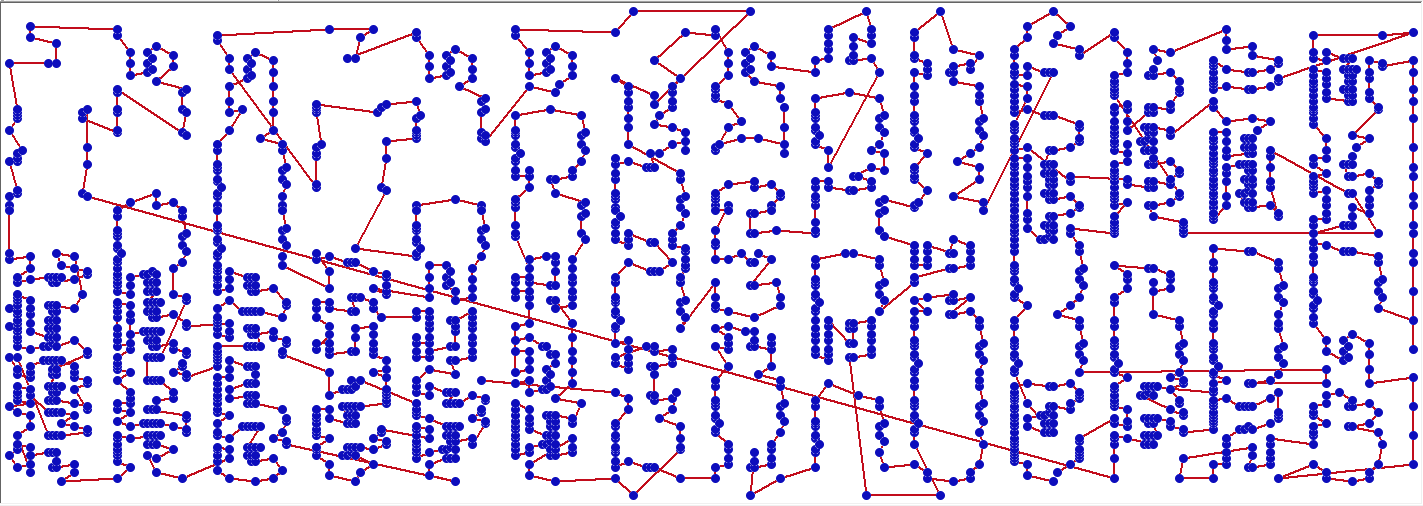
\includegraphics[width=\textwidth]{img/3/G.png}
      \caption{Greedy.}
    \end{subfigure}
    % \vspace{7mm}
    % \hfill
    \begin{subfigure}[t]{0.3\textwidth}
        \centering
        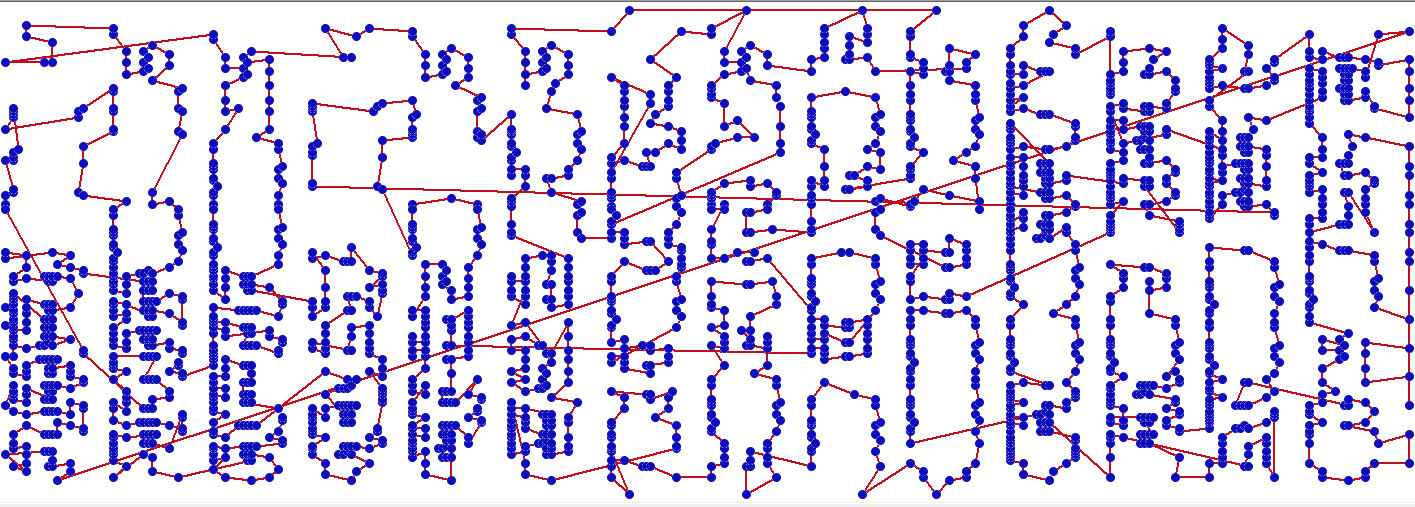
\includegraphics[width=\textwidth]{img/3/B.png}
        \caption{Borukva.}
    \end{subfigure}
    % \hfill
    \begin{subfigure}[t]{0.3\textwidth}
      \centering
      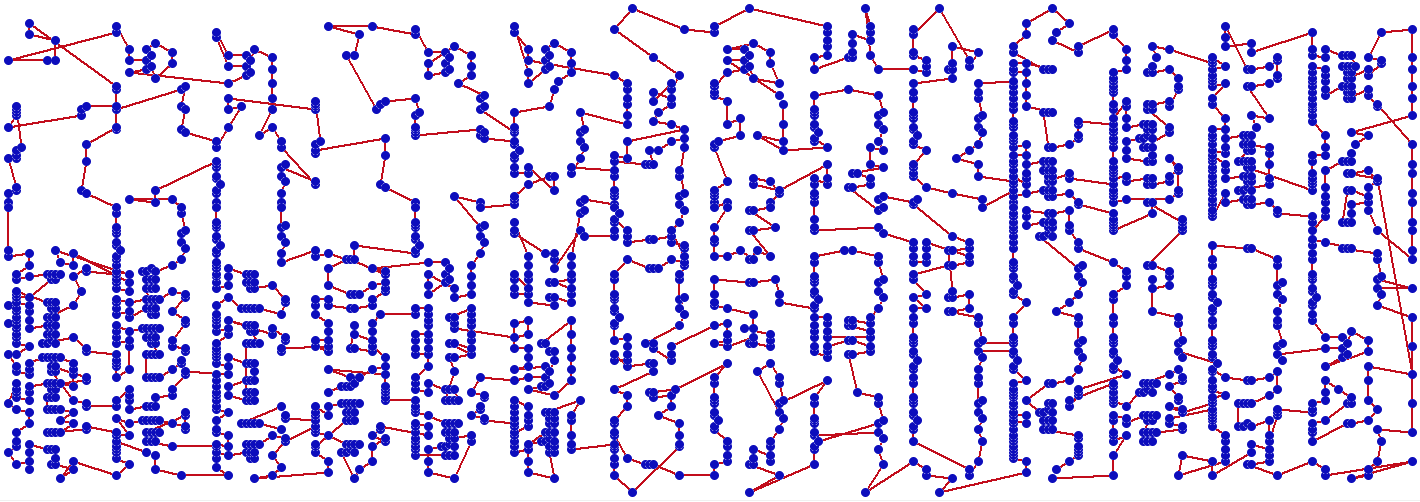
\includegraphics[width=\textwidth]{img/3/Q.png}
      \caption{Quick Borukva.}
    \end{subfigure}

    % \hfill
    \begin{subfigure}[t]{0.3\textwidth}
        \centering
        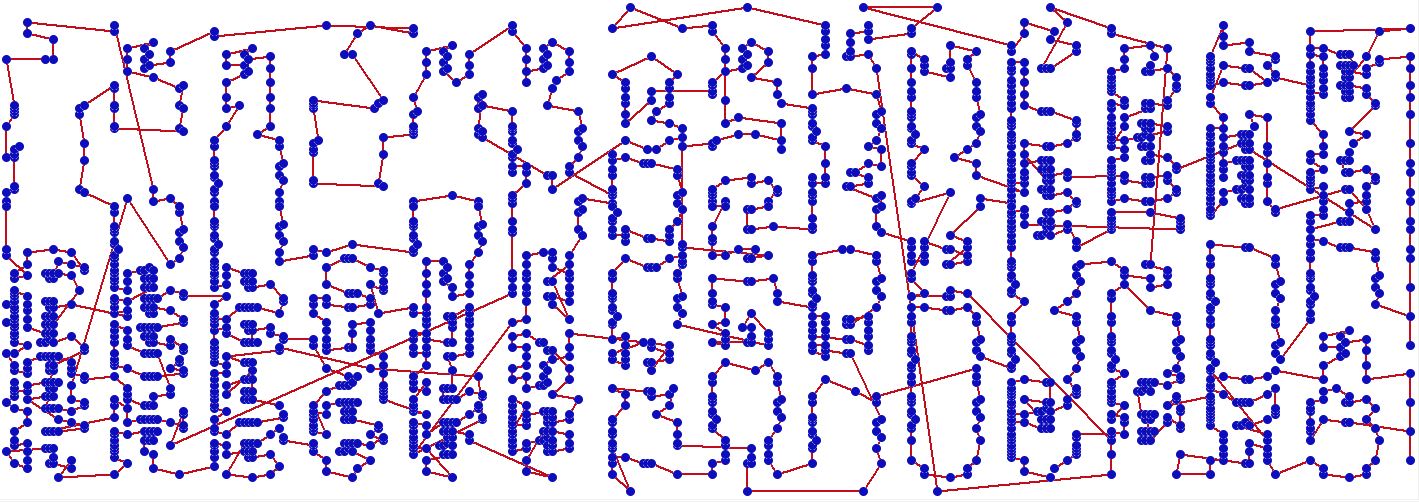
\includegraphics[width=\textwidth]{img/3/N.png}
        \caption{Nearest Neighbour.}
    \end{subfigure}
    % \hfill
    \begin{subfigure}[t]{0.3\textwidth}
        \centering
        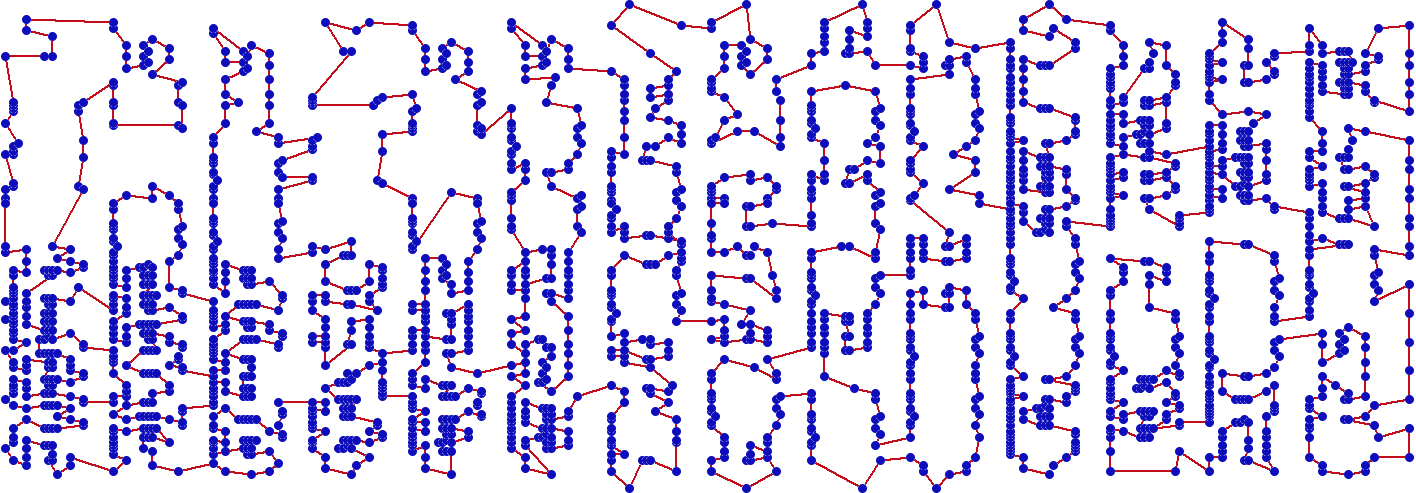
\includegraphics[width=\textwidth]{img/3/L1.png}
        \caption{Lin Kernighan Default.}
    \end{subfigure}
    % \hfill
    \begin{subfigure}[t]{0.3\textwidth}
        \centering
        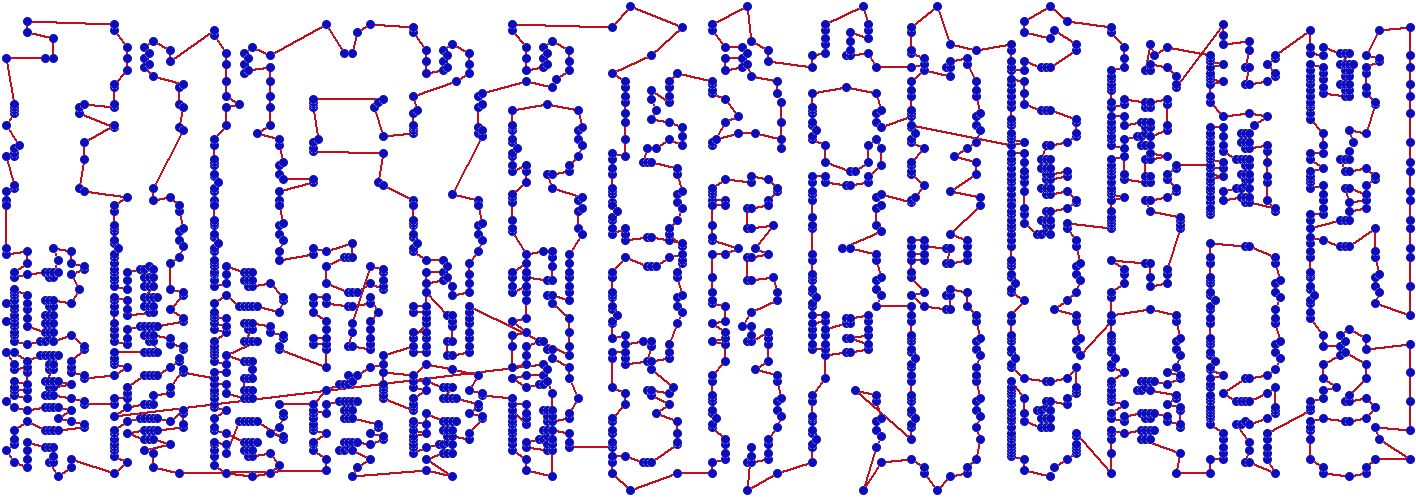
\includegraphics[width=\textwidth]{img/3/L10.png}
        \caption{Lin Kernighan 10 kicks.}
    \end{subfigure}

    % \hfill
    \begin{subfigure}[t]{0.3\textwidth}
        \centering
        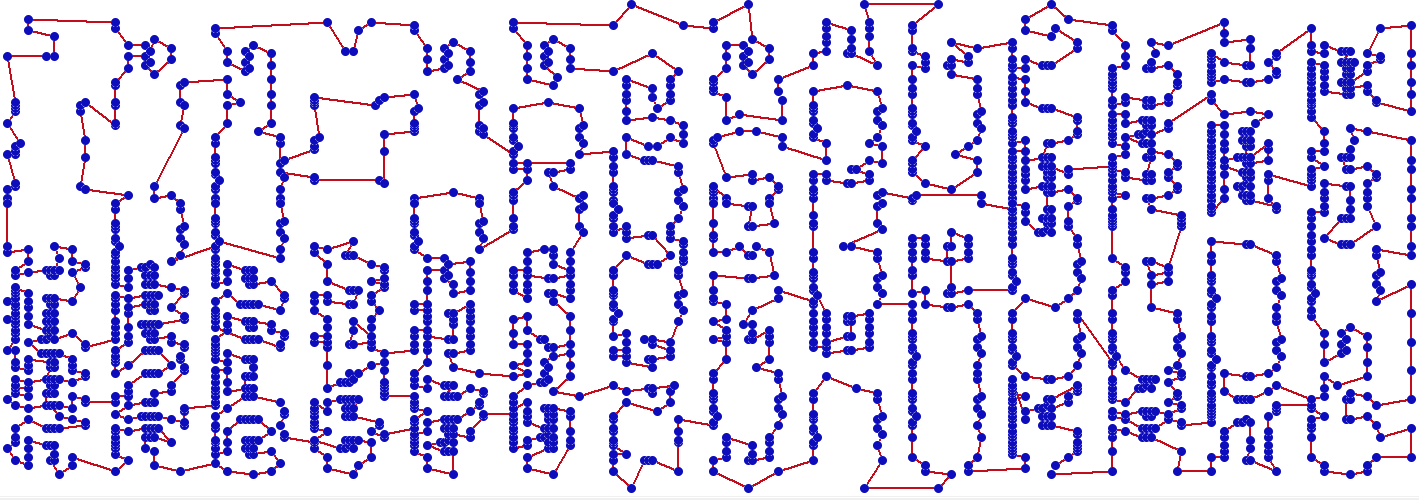
\includegraphics[width=\textwidth]{img/3/L100.png}
        \caption{Lin Kernighan 100 kicks.}
    \end{subfigure}
    % \hfill
    \begin{subfigure}[t]{0.3\textwidth}
        \centering
        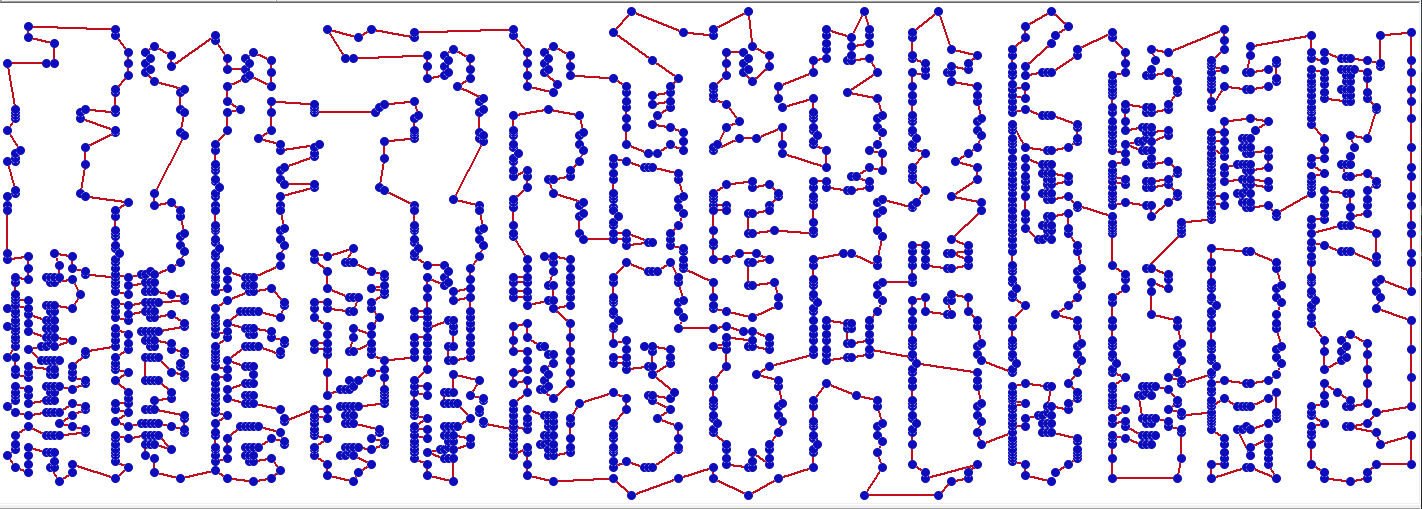
\includegraphics[width=\textwidth]{img/3/L+Q.png}
        \caption{L.K + Quick Borukva.}
    \end{subfigure}
    % \hfill
    \begin{subfigure}[t]{0.3\textwidth}
        \centering
        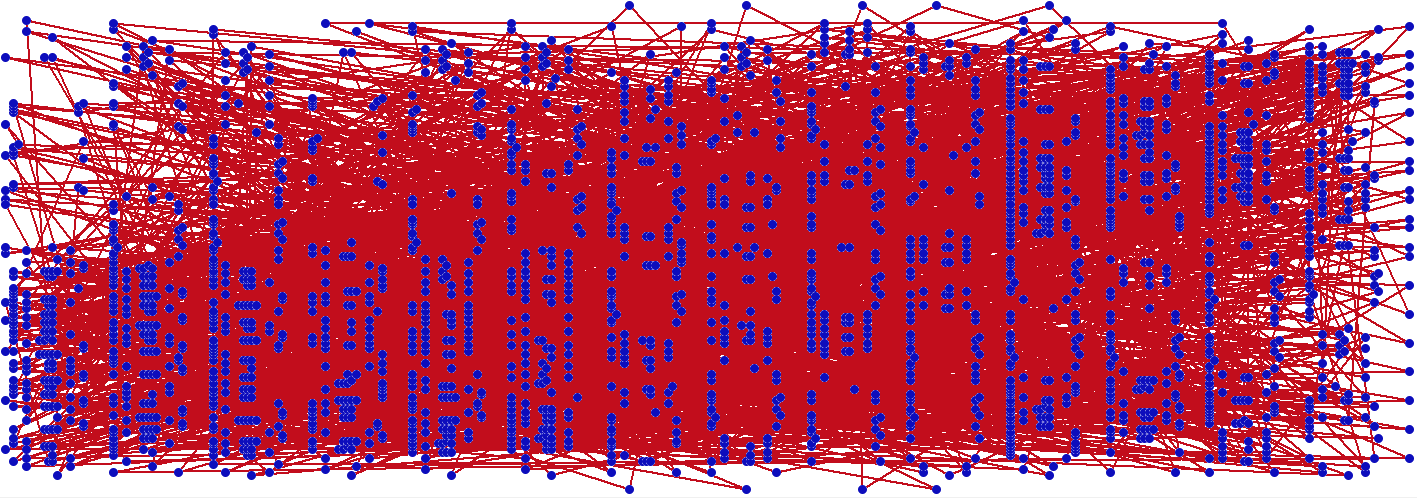
\includegraphics[width=\textwidth]{img/3/R.png}
        \caption{Random.}
    \end{subfigure}
    \caption{Rutas calculadas por cada heurística para el problema bck2217.}
\end{figure}

    % ==============================================================================
    \setlength{\parskip}{1em}
    \newpage
\end{document}

% ==============================================================================
% ==============================================================================